\chapter{Scientific Context}
\label{chap:scientific_context}
There have been many recent studies on the use of plasmas for sterilization and its effects on microorganisms \cite{bacteria, app_study, kit, wound,inactivation}. This chapter aims to provide an overview of the scientific context surrounding this topic, as well as research on the interaction of fungi with radiation.

The use of plasma treatment in the medical field goes back to the 20th century. Its history is outlined well in \cite{history}. While the first plasma treatments were used on skin their antimicrobial\footnote{Inhibits the growth of microorganisms.} properties were soon discovered. In the 1990s Mounir Laroussi demonstrated the use of dielectric barrier discharge (DBD) plasma for sterilization of surfaces \cite{laroussi}. Its first use focussed on the sterilization of medical instruments and equipment where removing bacteria and viruses is crucial. With this, many studies began on the interaction of plasma with bacteria, and it has been shown that DBD plasma can be used very effectively for sterilization \cite{inactivation, app_study}. As a result, many devices have been developed and are now commonly used in hospitals and laboratories \cite{history}. Although sterilization has been studied extensively most of the studies have focussed on the deactivation of bacteria exclusively. Recent studies have started to investigate the interaction of plasma with fungi which is relevant for the food industry and the cleaning of environments  \cite{growth}. While its efficacy has been proven well, it is not yet fully understood which processes carry responsibility for the inactivation of microorganisms especially on fungi. It is believed that the main mechanism of inactivation is the generation of reactive species in the plasma which can defuse into the cell and damage DNA and proteins \cite{app_study, inactivation}. A clear relationship between treatment time, proximity and inactivation rate has been shown. According to prior studies moulds like C. sphaerospermum are a lot more resistant to UV radiation than bacteria \cite{app_study}. 

Non-thermal plasma can, however, also radiate ultraviolet (UV) light, and the electric field applied through DBD can also have an effect on the microorganisms. A recent study by Li, Yiqian and others \cite{bacteria} has researched the effects of the physical energy of the plasma on bacteria by separating samples with different materials transparent to radiation and electric fields and found them to have a significant effect. In this work a similar approach is taken to investigate the effects of the radiation on the fungus C. sphaerospermum. The basis for which was formed by previous work by the department for plasma physics at the Kyoto Institute of Technology done by Tomoya Ohara and others \cite{kit}. They showed that treatment times of 20 minutes are sufficient to inactivate the fungus by more than 99 \% and measured the concentration of ozone and hydroxide ions. Figure \ref{fig:kit} shows the results of their study.

\begin{figure}
    \centering
    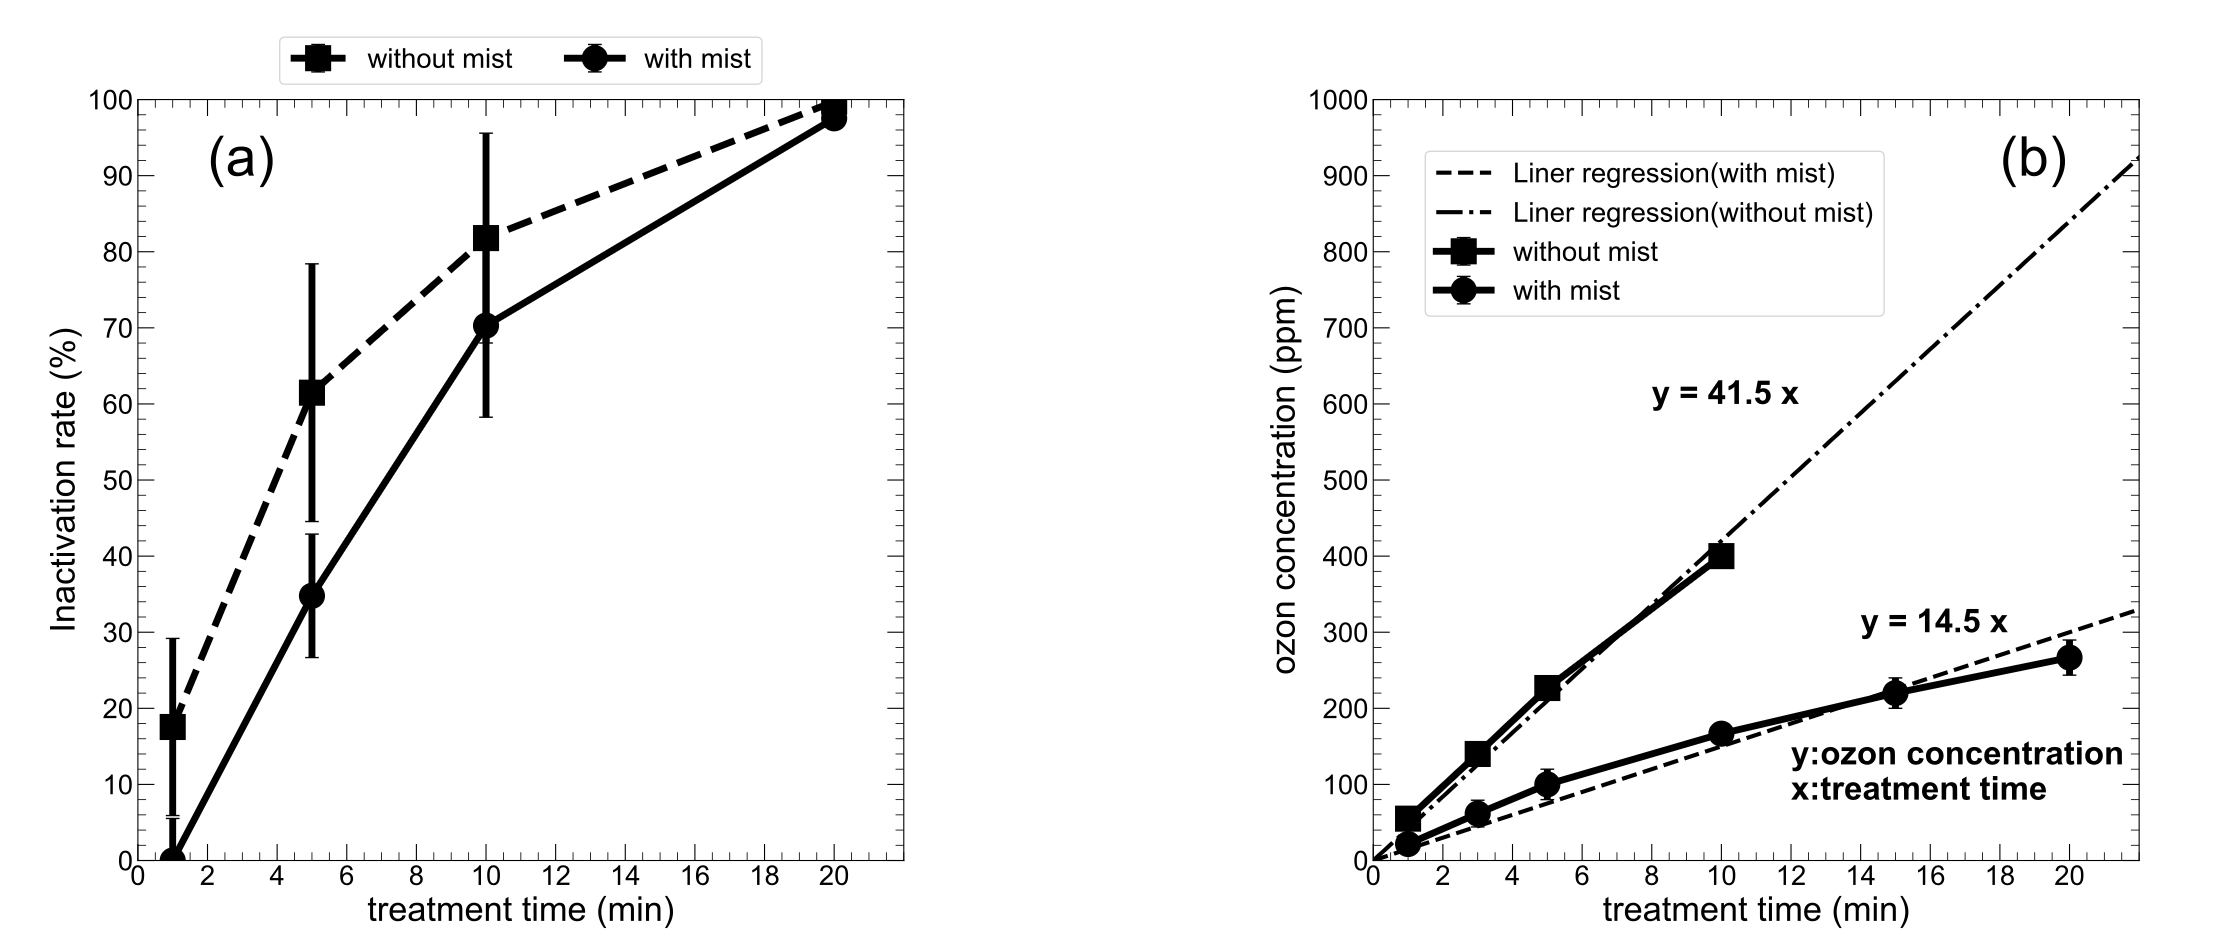
\includegraphics[width=1\textwidth]{images/KIT_work.png}
    \caption[Results of the study by Tomoya Ohara and others]{Results of the study by Tomoya Ohara and others \cite{kit}. (a) inactivation rates of C.sphaerospermum as a function of treatment time in the
    treatments without and with water mist, and (b) ozone concentration as a function of the
    time.}
    \label{fig:kit}
\end{figure}
